\thesischapter{Simulating and Verifying the European Rail Traffic Management System Using Real Time Maude}{Simulating and Verifying the European Rail Traffic Management System Using Real Time Maude}\label{chapter:verifyertms}\label{chap:verifyertms}
\chaptermark{Simulating and Verifying ERTMS using Real Time Maude}


In the following we describe how the Real Time Maude tool can be used to analyse the performance and safety of the ERTMS system by both simulation and verification using the Maude LTL model checker (The modelling of ERTMS in Real Time Maude was describe in Chapter~\ref{chap:modelertms}).  We begin by presenting the simulation of the pentagon example which demonstrates a situation where a slow train is held up by a faster train. Secondly we look at applying model checking to both the pentagon example and the junction example. The safety properties verified for the pentagon example relate to the safety condition "The movement authorities of the two trains do not overlap" whilst the properties for the junction example relate to the safety condition "The point does not move when it is in a train's movement authority". We also modified the pentagon example to use more realistic distances (See Section~\ref{sec:executionofltlchecker}). 

It is stated by its developers that Real Time Maude is not first and foremost a verification tool. This is due to some inherent limitations in LTL-model checking that hinder the verification of infinite state systems. We have, as in the sensor network example \cite{PO07}, only model checked a portion of the state space for the pentagon. This is however enough to have confidence in the correctness of the system with respect to a given safety condition. A larger portion of the state space could be model checked by removing non-determinism from the model making it more concrete. This has been done in the junction example where the radio block processor is modified in such a way that it processes movement authorities in one time step.


\section{Simulating The Behaviour of ERTMS}

We will now see how this executable specification can be used to simulate and analyse the performance of the modelled system. Simulation of the system up to a given time $n$ is achieved by rewriting the initial state of the system to each of the intermediate time steps $0 \ldots n$. A simple Haskell program has been written that can parse the output of each step, extract the relevant data and then plot a graph.

We use an initial state containing two trains one of which is slower (train1) than the other (train2), an interlocking and a radio block processor. The faster train will eventually catch up with the slow train and it waits for that train to clear all successive track segments before proceeding. The trains start at positions on opposing sides of the track with train1 starting at 0 and train2 starting at 150. The RBC and the interlocking are both initialised with the trains in these positions. In Maude this initial state is modelled as follows. Firstly, we define the initial states of the component objects individually:

\begin{lstlisting}[caption = The initial interlocking state in Maude]
 eq initialintstate2 = < inter1 : Inter | state : idle, 
                         reqid : 0, t0 : true, 
                         t1 : false, t2 : false, 
                         t3 : true, t4 : false > .
\end{lstlisting}

The  interlocking is initially idle, the request variable is set to zero, the track segments containing trains are set to true and the remaining track segments are set to false.

\begin{lstlisting}[caption = The initial RBC state in Maude]
 eq initialrbcstate2 = < rbc1 : RBC | state : rbcidle, 
                         lasttrain : train1,  
                         ma : (train1 |-> 49, train2 |-> 199), 
                         pos : (train1 |-> 0, train2 |-> 150), 
                         curreq : empty > .
\end{lstlisting}

Like the interlocking, the RBC is also initially idle. Since the \texttt{lasttrain} variable has not effect in this state and will be set in any successive control flow we simply set it to be train1. The movement authorities  and positions of the trains are set within the ma and pos mapping respectively and the current request is empty.  

\begin{lstlisting}[caption = The intital state of train1 in Maude]
 eq initialtrainstate1 = < train1 : Train | state : acc,  dist : 0, 
                           speed : 1, ac : 1, ma : 49, 
                           tseg : 0, maxspeed : 4 > .
\end{lstlisting}
We set the train1 to be accelerating initially with a distance and speed of 0. Its movement authority is 49, it is in the 0 track segment and has a maximum speed of 4. 

\begin{lstlisting}[caption = The intial state of train2 in Maude]
eq initialtrainstate2  = < train2 : Train | state : acc, dist : 150, 
                           speed : 1, ac : 1, ma : 199,
                           tseg : 3, maxspeed : 7 > .
\end{lstlisting}
Like train1, train2 is also accelerating initially and has a speed of 0.  Unlike train1 it has a distance of 150, a movement authority of 199, it is in the 4th track segment number 3 and has a maximum speed of 7. Both trains have an acceleration of 1. 

Using these initial states for the individual objects we can form the initial state for our pentagon example using the following command:
\begin{lstlisting}
 eq initialstate2 = {initialtrainstate1 initialtrainstate2 
                         initialintstate2  initialrbcstate2} . 
\end{lstlisting}
The operation \texttt{initialstate2} is of type \texttt{System} and contains a \texttt{Configuration} consisting of the initial states of train1, train2, the RBC and the interlocking. This initial state forms a model of ERTMS which we can simulate using Real Time Maude to rewrite it to a state after a set number of time steps. The model of ERTMS is executed using the following command:
\begin{center}
\texttt{(trew initialstate2 in time $\leq$ 50 .)}
\end{center}

In the resulting output at time 50 both of the trains have moved a considerable distance with train1 (See line 9 of Code Listing \ref{cl:initialstate2rewrite}.) moving to distance 184 and train2 moving to distance 128. Both trains have also requested and received new movement authorities.
 
\begin{lstlisting}[caption = The result of rewriting initialstate2 for 50 time steps, label = cl:initialstate2rewrite]
Result ClockedSystem :
  {< inter1 : Inter | reqid : 3,state : idle,
     t0 : false,t1 : false,t2 : true,
     t3 : true,t4 : false > 
   < rbc1 : RBC | curreq : train2,lasttrain : train2,
     ma : (train1 |-> 199, train2 |-> 149),
     pos : (train1 |-> 180, train2 |-> 122),
     state : rbcidle > 
   < train1 : Train | ac : 1,dist : 184,ma : 199,maxspeed : 4,
    speed : 4,state : cons,tseg : 3 > 
   < train2 : Train | ac : 1,dist : 128,ma :
    149,maxspeed : 7,speed : 5,state : break,tseg : 2 >} in time 50
\end{lstlisting}

\begin{figure}

\begin{center}
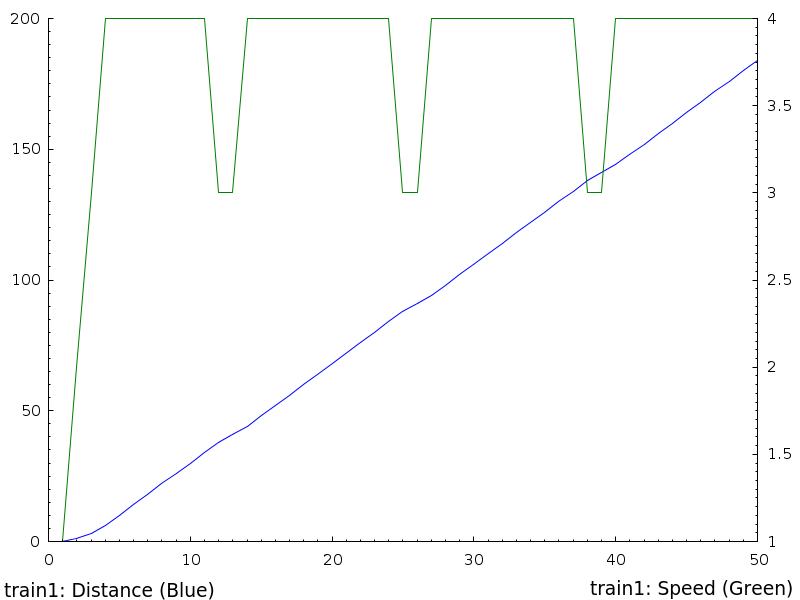
\includegraphics[scale=0.5]{t1graph.png}
\end{center}
\caption{A graph comparing the distance and speed of train1}
\label{t1graph}
\end{figure}

\begin{figure}

\begin{center}
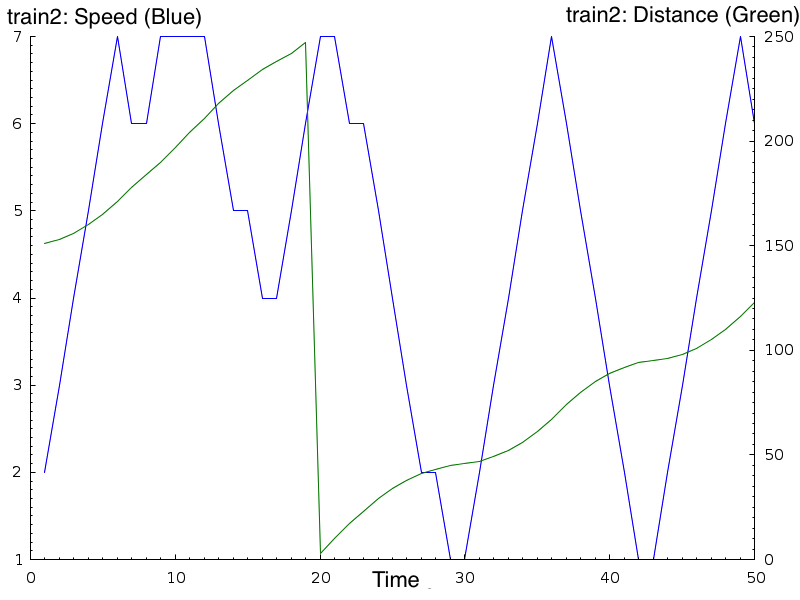
\includegraphics[scale=0.5]{t2graph.png}
\end{center}
\caption{A graph comparing the distance and speed of train2}
\label{t2graph}
\end{figure}

\begin{figure}

\begin{center}
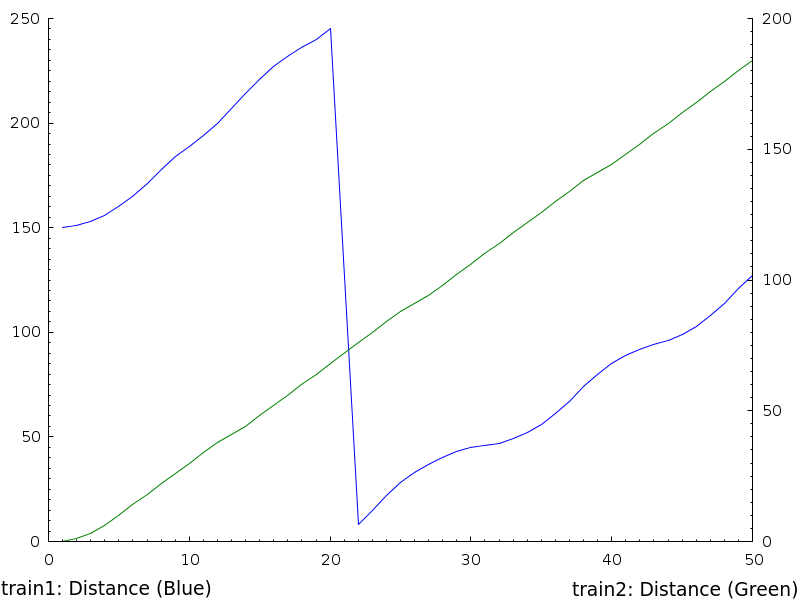
\includegraphics[scale=0.5]{t1t2graph.png}
\end{center}
\caption{A graph comparing the distances of train1 and train2}
\label{t1t2graph}
\end{figure}

The first graph (See Fig. \ref{t1graph}.) shows the speed and distance of train1 over time. The train spends the majority of its time at maximum speed however there is a slight decrease in speed when a movement authority is requested. The distance of the train increases in roughly a linear fashion. The second graph (See Fig. \ref{t2graph}.) shows the speed and distance of train2 over time. The train brakes repeatedly and at one position comes to a complete stop as it waits for the slower train to progress and exit its current track segment. The distance time graph shows this stop/start behaviour through a wavy appearance. The final graph (See Fig. \ref{t1t2graph}.) shows that there is a consistent distance between the two trains of at least one track segment. Due to the discretisation of time we have had to favour braking over accelerating in order for the train to stop behind its movement authority. The speed of the train decreases on a transition from accelerating or full speed states to a braking state but does not increase speed immediately on a transition from a braking to accelerating state. This behaviour can be see in the speed graph for train2 (See Fig. \ref{t2graph}.) where there are several sharp peaks where the maximum speed has only been in place for one time step. In contrast when the train transitions from braking to accelerating there is always a flat section of constant speed. These flat sections of constant speed also occur when the train is braking and the train jumps back into the accelerating state for one time step to ensure the train brakes as closely to the end of movement authority as possible.


\section{The Maude Linear Temporal Logic Model Checker}
The Real Time Maude system employs the Maude LTL Model Checker, which does on-the-fly model checking (See Chapter~\ref{chapter:modelchecking}), for \cite{ES00} verification purposes.  This is a useful automatic tool which allows for the verification and analysis of real time systems. In addition to the positive verification results in which a safety property holds,  the system produces, in the case of a negative verification result, a counterexample trace which describes how the error occurred from the initial state of the system.

 

\section{Model Checking the European Rail Traffic Management System}
In the following section we will demonstrate an approach to apply the Real Time Maude LTL model checker to verify the Real Time Maude specification described previously.
Firstly we shall define the property we want to check in the Real Time Maude system. To do this we have to define a satisfaction relation which describes what it means for the property to hold in a state of the system we are checking. The property we shall consider in this case is that the moment authorities of two trains in the system do not overlap. The logical property we define identifies the individual trains using their object identifiers and then computes whether or not an overlap has occurred using a Boolean formula.  We shall show that it is possible to verify this property over a time period large enough for all normal behaviours of the system to occur. 

\subsection*{Defining a Satisfaction Relation}
The syntax of the properties for which we are going to check using the LTL model checker are defined separately from the semantics in terms of a satisfaction relation.
We shall now describe how to define the behaviour of the satisfaction relation for a given system and property as a Real Time Maude specification. The satisfaction relation itself is predefined in a specification as an operation which takes a State and a property which is of type Prop and computes a Boolean. Maude defines the satisfaction relation $\models$ in the following:
\medskip

\begin{lstlisting}[caption =  The Maude Satisfaction module, label =code:satisfaction ]
  fmod SATISFACTION is  
    protecting BOOL .  
    sorts State Prop .  
    op _|=_ : State Prop -> Bool [frozen] .  
  endfm
\end{lstlisting}
\medskip
The sorts \texttt{State} and \texttt{Prop} are undefined as is the behaviour of $\models$. It is left to the user of the model checker to define the behaviour for their own purposes. The standard way to define predicates which refer to a given object is by pattern matching object identifiers. We have added general rules to deal with terms containing the operations \texttt{delta} and \texttt{trackseg}. In both cases the operation is ignored and the property is checked on the term without the operations.

\begin{lstlisting}[caption = Rewriting rules to deal with delta and trackseg operations]
var P : Prop .
eq {delta(REST)REST2} |= P = {REST REST2} |= P .
eq {trackseg(REST)REST2} |= P = {REST REST2} |= P .
\end{lstlisting}

\subsection*{Checking the  Correctness of the Specification}

We have applied model checking to check several fundamental correctness properties of the pentagon example's behaviour. We begin by showing that it is not possible for a train to exceed its maximum speed. We formulate this as a model checking problem over the pentagon example.  We can check that a train has a certain speed as follows:

\begin{lstlisting}[caption = The speed property]
op train-s : Oid Nat -> Prop [ctor] .
eq {REST < O1 : Train | speed : N1 >} |= train-s(O1,N1') = 
   (N1 == N1')  .
\end{lstlisting}

Here the natural number \texttt{N1} in the train object is matched with \texttt{N1'} in the predicate \texttt{train-s}. This can be used to state that train1 does not exceed its maximum speed in any state in the pentagon  example that is reachable in 100 time steps using the following command:

\begin{center}
\texttt{(mc initialstate2 |=t  ~(<> train-s(train1,5)) in time <= 100 .)}
\end{center}

The resulting output from the model checker shows that the property has been proven true in 230 seconds:

\begin{lstlisting}[caption = The result of model checking the max speed property for train1 ]
rewrites: 66202099 in 229900ms cpu (229901ms real) 
(287960 rewrites/second)
Model check initialstate2 |=t ~ <> train-s(train1,5)
in MODEL-CHECK-ERTMS8 in time
  <= 100 with mode deterministic time increase

Result Bool : true
\end{lstlisting}

We will now show that the train is always at the correct speed for the cons and stopped states. This is formulated using two properties. We can check that a train is in a specific state, in this case the \texttt{cons} state, as follows:

\begin{lstlisting}[caption = The cons state property]
ops train-cons : Oid -> Prop [ctor] .
eq {REST < O1 : Train | state : S >} |= train-cons(O1) 
   =  S == cons . 
\end{lstlisting}


This predicate holds if there is a train in the configuration with object identifier O1 and a state cons. 

We can use these two properties and others formulated in a similar fashion to formulate model checking properties which can be used to check the correctness of our modelling approach. We can define three safety conditions, one that states "train1 is in the cons state if and only it is at it's maximum speed". The second states "if the speed of train1 is zero then it is either in the cons, stop or acc states and if the train is in the stop state then it's speed is zero". The final states "it is not the case that there exists a state in which the speed of train1 is 5" (train1 has a maximum speed of 4). 

\begin{lstlisting}[caption = The model checking commands for the correctness properties ]
Correct1 := (mc initialstate2 |=t  
  ~(<> train-s(train1,5)) in time <= 100 .)
Correct2 := (mc initialstate2 |=t 
  [] (train-s(train1,4) => train-cons(train1)) /\ 
     (train-cons(train1) => train-s(train1,4))  
  in time <= 100 .)
Correct3 := (mc initialstate2 |=t [] ((train-s(train1,0) => 
  (train-stop(train1) \/ train-brake(train1) \/ train-acc(train1))) 
   /\ (train-stop(train1) => train-s(train1,0))) in time <= 100 .)
\end{lstlisting}

\subsection*{Defining "No Overlapping Movement Authorities"}
We verify the safety condition "The movement authorities of two trains do not overlap" by model checking three safety properties MA1, MA2 and MA3 that correspond to checking the different possible safe positions over movement authorities and trains on the track. To do this we define a satisfaction relation for two Maude operations of type $\mathbf{Prop}$ which capture each of these safety properties. The first of these can be seen below:

\begin{lstlisting}[caption = The no overlapping movement authorities property]
eq {REST < O1 : Train |  dist : D1 , ma : M1 > 
   < O2 : Train |  dist : D2 , ma : M2 >} |= nomaoverlap1(O1',O2') = 
   (O1 == O1') and (O2 == O2') and noolap1(D1,M1,D2,M2) .
\end{lstlisting}

Here we have matched two object identifiers and natural numbers and called a Boolean function \texttt{noolap} on those variables. This definition features an external operation which computes a Boolean depending on whether a set of inequalities is satisfied. The three sets of inequalities corresponding to the three safety properties are defined below:

\begin{lstlisting}[caption = The no overlap operations]
eq noolap1(D1,M1,D2,M2) = 
    (D1 <= M1) and (D2 <= M2) implies ((M1 <  D2) or (M2 < D1)) .  
eq noolap2(D1,M1,D2,M2) = 
    ((M1 < D1) and (D2 <= M2)) implies (M2 < D1 and M1 < D2) .
eq noolap3(D1,M1,D2,M2) = 
    ((M2 < D2) and (D1 <= M1)) implies (M1 < D2 and M2 < D1) .

\end{lstlisting}

There are four possible combinations of trains and movement authorities.  The first case is that train one is behind it's movement authority which is behind the second train which itself is behind it's movement authority. The second case is the reverse of the first case. In the third and fourth cases  one of the trains is behind it's movement authority and the other is towards the end of the track and has its movement authority extended into the initial segment at the beginning of the track.


\subsection*{Defining "A Point Does Not Move"}
We formalise the safety property "a point does not move when it is in a movement authority" as two safety conditions. The first states that it is globally true that if the point is in the movement authority of train1 then the point is set to normal. The second states that it is globally true that if the point is in the movement authority of train2 then the point is set to reverse. These two safety conditions were formalised using three Maude operations of type $\mathbf{Prop}$. $\mathbf{pointma}$ is used to compute whether the point is in the movement authority of a train; $\mathbf{pointnormal}$ and $\mathbf{pointreverse}$ cause the satisfaction relation to hold if the point is in the position corresponding to the property. 

\begin{lstlisting}[caption = The point properties]
  eq { REST  < O1 : Train |  dist : D1 , ma : M1 > } |= pointma(O1) 
      =  ptma(D1, M1)  .
  eq { REST   < O1 : Inter | p1n : B >  } |= pointnormal = B .
  eq { REST   < O1 : Inter | p1r : B >  } |= pointreverse = B .
\end{lstlisting}

\subsection{Execution of The LTL Model Checker}\label{sec:executionofltlchecker}

We shall now describe the execution of the Maude LTL model checker in Real Time Maude. This is done using the \texttt{mc} command with some initial state of type \texttt{System}, a satisfaction relation, the LTL formula to be checked and an optional time. The satisfaction relation can be either $\models_u$ for un-timed model checking for which time is not specified or $\models_t$ for which the optional time is specified.

The Maude LTL model checker is then called using the following command:

\begin{center}
\texttt{(mc initialstate2 |=t [] nomaoverlap1(train1,train2) in time <= 100 .)}
\end{center}
The command states that we are applying timed model checking to check that it is globally true that the movement authorities of the trains do not overlap at all moments in time less than or equal to 100. This results in the following output from Real Time Maude which indicates that the property was successfully verified in 1 minutes and 32 seconds taking the system approximately 76 million rewrites.
\begin{lstlisting}[caption = No overlapping movement authorities model checking result]
rewrites: 76099490 in 91776ms cpu (91776ms real) 
(829187 rewrites/second)
Model check initialstate2 |=t[]nomaoverlap1(train1,train2)
in MODEL-CHECK-ERTMS8
   in time <= 100 with mode deterministic time increase

Result Bool : true
\end{lstlisting}

Unfortunately the Maude LTL model checker cannot detect the congruence between difference configurations of control system. Therefore the state space is infinite and it is impossible to do un-timed model checking on the above model checking problem for the pentagon example. It is however possible to do timed model checking within a reasonable time limit that allows for all behaviours of the system to be verified. The junction example does not suffer from this problem as the state space is finite and, in addition, it has additional mechanisms to remove non-determinism from the model which dramatically cuts down on the state space.

The following command is used to model check the safety property P1 for the junction example.

\begin{lstlisting}[caption = The model checking command the point does not move property]
(mc initialstate1 |=u [] (pointma(train1) => pointnormal)  .)
\end{lstlisting}

\section{Results}
The following table presents the times taken to verify the three correctness properties and five safety properties MA1, MA2, MA3, P1 and P2:
\medskip
\begin{center}
\begin{tabular}{c | c | c} 
Safety Condition & Time Steps Checked & Time to Solve  \\ \hline
Correct1 & 100 & 229.400 s\\
Correct2 & 100 & 249.784s\\
Correct3 & 100 & 225.556s\\
MA1 (Pentagon)& 100 & 91.756s  \\
MA2 (Pentagon)& 100 &129.335s \\ 
MA3 (Pentagon)& 100 &148.032s \\
P1 (Junction)& untimed &7.488s \\
P2 (Junction)& untimed & 6.636s \\
\end{tabular}
\end{center}
\medskip
The removal of non-determinism from the pentagon example has made timed model checking more successful. Prior to the \texttt{nondelta} operation (See Chapter~\ref{sec:maudetimemodelling}) being added the safety properties could only be checked for the first 30 time steps of the system.

The no overlapping movement authorities safety property was verified using time bounded model checking over the modified realistic pentagon example with a track segment length of 25000,  segment length of 5000 and train speeds of 70 and 120.  We then applied the LTL model checker and verify this example so that a comparison can be performed between the two pentagon examples in terms of verification difficulty.. The following table shows how the difficulty of the model checking problem increases with search depth:
\medskip
\begin{center}
\begin{tabular}{c | c | c} 
Safety Condition & Time Steps Checked & Time to Solve  \\ \hline
MA1 (Realistic Pentagon) & 30 & 25.265s \\
MA1 (Realistic Pentagon) & 40 & 36.414s \\
MA1 (Realistic Pentagon) & 50 & 49.201s \\
MA1 (Realistic Pentagon) & 60 & 62.126s \\
MA1 (Realistic Pentagon) & 70 & 79.948s \\
\end{tabular}
\end{center}
\medskip
Even though the Real Time Maude system is unable to perform un-timed model checking on this example it can still perform bounded model checking of a large enough portion of the state space for us to be satisfied that the system is safe.

\section{Future Work}
There are numerous ways in which our model can be extended. One of the biggest problems facing engineers when developing the ERTMS system is time and how it affects the transition of messages with delays often occurring. This could be easily modelled following the work \cite{PO07} where delays are modelled in the communications between nodes of a wireless sensor network. Currently our trains have a jerky behaviour in terms of speed, breaking and accelerating in rapid succession and there are several other behaviours that trains exhibit in real life that we have not captured in our model. For example, trains have the ability to coast where the engine in not powering the train but the brakes are not active which is used for several purposes. To save energy coasting and accelerating are often combined to hold the train at an optimum speed. The trains may also coast before breaking when reaching the end of a movement authority. The RBC has the possibility to pre-emptively grant movement authorities to trains without them requesting it in the case that a train is on a route which contains free sections of track behind a movement authority.  The trains could also request movement authorities before the point at which we reach the braking point.

\begin{comment}
Currently the track is closed and trains are capable of looping round the track giving it a very large state space due to number of possible combinations of train location and speed. Opening up the track with an entrance and exit would provide the opportunity to model the hand over part of the protocol where new trains must register with the RBC on entering the track and then de-register upon leaving. This would  This example could then be extended by increasing the complexity of the track further and then modelling routes and points. This would allow for the checking of a further safety conditions that states no train has a movement authority over a point in locked in the wrong direction or a moving point.
\end{comment}
It is highly desirable to be able to verify properties about the energy consumption of the ERTMS and traditional railway control systems and prove that the former is more efficient than the latter. It is also desirable to verify properties of the systems performance in a similar fashion; our current model provides a framework for this.

The next challenge would be to verify  some real world track layouts as would be controlled by the ERTMS system on its implementation. This would require further removal of non-determinism from the models and a more general approach to modelling the railway interlocking. A summer project student at Swansea University has successfully modelled an interlocking, which acts as a ladder logic interpreter, and executes a ladder logic program. This could be integrated with our model and would allow for a general approach to model tracks, rather than having to model each interlocking by hand.

